\documentclass[12pt,twoside]{article}
\usepackage[dvipsnames]{xcolor}
\usepackage{tikz,graphicx,amsmath,amsfonts,amscd,amssymb,bm,cite,epsfig,epsf,url}
\usepackage[hang,flushmargin]{footmisc}
\usepackage[colorlinks=true,urlcolor=blue,citecolor=blue]{hyperref}
\usepackage{amsthm,multirow,wasysym,appendix}
\usepackage{array,subcaption} 
% \usepackage[small,bf]{caption}
\usepackage{bbm}
\usepackage{pgfplots}
\usetikzlibrary{spy}
\usepgfplotslibrary{external}
\usepgfplotslibrary{fillbetween}
\usetikzlibrary{arrows,automata}
\usepackage{thmtools}
\usepackage{blkarray} 
\usepackage{textcomp}
\usepackage[left=0.8in,right=1.0in,top=1.0in,bottom=1.0in]{geometry}
\newcommand{\rnd}{\Tilde}
\newcommand{\ru}{\rnd{ u}  }
\newcommand{\rd}{\rnd{ d}  }
%\newcommand{\rs}{\rnd{ s}  }
\newcommand{\ri}{\rnd{ i}  }
\newcommand{\re}{\rnd{ e}  }
\newcommand{\rQ}{\rnd{ q}  }
\newcommand{\rC}{\rnd{ c}  }
\newcommand{\rX}{\rnd{ x}  }

\usepackage{pdfpages}


\title{Probability and Statistics For Data Science HW 6}
\author{gjd9961}
\date{November 2021}
\begin{document}
\maketitle
\begin{enumerate}

\item (Bayesian coin flip)
Let us try out another prior for the Bayesian coin flip problem in the notes. We now model the parameter of the Bernouilli as being uniform between $1/2$ and $1$.
\begin{enumerate}
\item Briefly justify the model and compute the probability that the result of the coin flip is heads or tails under this model. 
\subitem
We use the parameter $\theta$ to represent the probability of a coin flip being heads. Because our uncle is a tricketer, and we assume that he's stacking the odds in his favor, we assume that the coin must be weighted in his favore. Therefore, it is reasonable to assume that the odds the coin flip being heads is greater than $\frac{1}{2}$, and since probabilities only go from 0 to 1, then the range of $\theta$ is $\frac{1}{2} \leq \theta \leq 1$. Now lets compute the probability of a heads, and the probability of a tails, assuming theta is uniformly distributed along its range.
\begin{equation}
    \begin{split}
        P(\rX=heads) &= \int_{.5}^1 f_\theta(\theta) \times P(heads|\theta) d\theta \\
        P(\rX=heads) &= \int_{.5}^1 2\theta \\
        P(\rX=heads) &= 1-.25 = .75  \\
        \text{And } & \\
        P(\rX=Tails) &= 1 -.75 = .25
    \end{split}
\end{equation}
We know that $f_\theta(\theta)$ is equal to the density at that point, which is equal to 2, since our $\theta$ is uniformly distributed along $.5 \leq \theta \leq 1$. Likewise, the probability of flipping a heads given a $\theta$ is just $\theta$. 

\item After the coin flip we update the distribution of the bias of the coin (i.e. the parameter of the Bernouilli that represents the coin flip) by conditioning it on the outcome. Compute the distribution if the outcome is tails and if the outcome is heads. Sketch any distributions you compute and explain why the drawing makes sense.
\subitem 
In this problem, we will update our beliefs about the fairness of the coin given some assumptions about the coin and data collected on flips. In this way, we condition on the prior events to calculate a posterior probability. We will need to calculate two posteriors, one for theta if we flip a heads, (which should assign higher probability to greater degrees of favor to landing on heads), and one for theta if we flip a tails, (one which should assign higher probability to the coin being closer to fair). We do so as follows:

\begin{equation}
    \begin{split}
        f(\theta|heads) &= \frac{f_\theta(\theta)\times P(heads|\theta)}{P_{\rX}(heads)} = \frac{2\theta}{\frac{3}{4}} = \frac{8\times \theta}{3} \text{ for }\frac{1}{2} \leq \theta \leq 1 \text{ otherwise } 0 \\
        \text{And} & \\
        f(\theta|tails) &= \frac{f_\theta(\theta)\times P(tails|\theta)}{P_{\rX}(tails)} = \frac{2(1-\theta)}{\frac{1}{4}} = 8-8\times\theta \text{ for }\frac{1}{2} \leq \theta \leq 1 \text{ otherwise } 0 \\
    \end{split}
\end{equation}
\begin{figure}[h!]
    \centering
    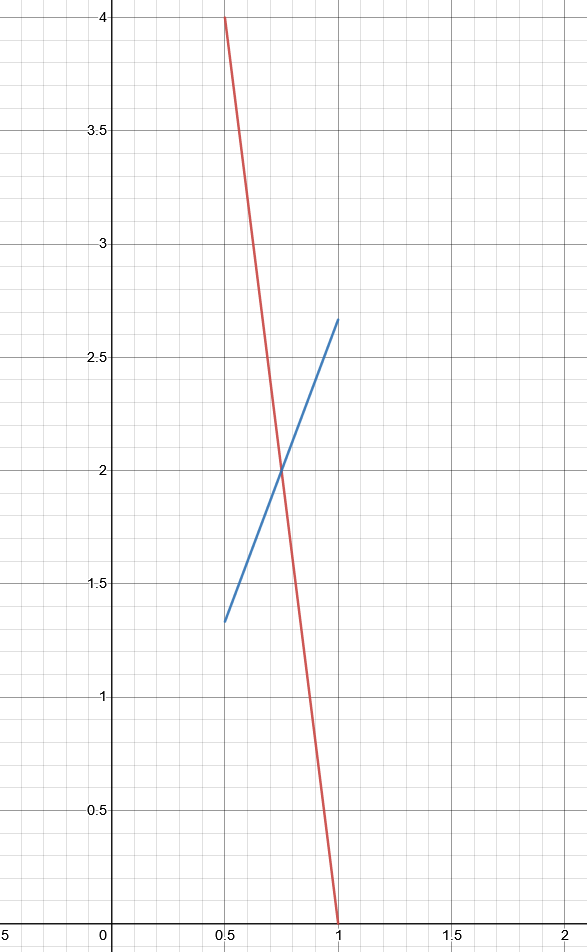
\includegraphics[scale=.4]{hw6 desmos 1.b.png}
    \caption{Posteriors of Theta Given Heads (Blue) or Tails (Red)}
    \label{fig:my_label}
We can see that the flip verifies our assumptions about how the distribution of should change: the area under the red line is higher for $\theta\leq.75$ and the opposite is true for the blue line.
\end{figure}
\item You observe 100 coin flips and they all turn out to be tails (i.e. 0). Do you think you should reconsider your prior? If so, why?
\subitem
Yes we definitely should reconsider our priors. If we performed MLE given our data, by tweaking $\theta$ in the range we defined ($.5\leq \theta \leq1$), the most likely $\theta$ would be $\frac{1}{2}$ and the probability of the event occurring would be $(\frac{1}{2})^{100}$ which is incredibly unlikely. Our assumptions are too rigid, and because we defined our range for $\theta$ we will never have non-zero probability of the coin having parameter $\theta < .5$, which means we should definitely reconsider our assumptions.
\end{enumerate}

\item (Halloween parade)
The city of New York hires you to estimate whether it will rain during the Halloween parade. Checking past data you determine that the chance of rain is 20\%. You model this using a random variable $\rnd{r}$ with pmf
\begin{align*}
 p_{\rnd{r}}(1) = 0.2, \qquad p_{\rnd{r}}(0)=0.8,
\end{align*}
where $\rnd{r}=1$ means that it rains and $\rnd{r}=0$ that it doesn't. Your first idea is to be lazy and just use the forecast of a certain website. Analyzing data from previous forecasts, you model this with a random variable $\rnd{w}$ that satisfies 
\begin{align*}
 P(\rnd{w}=1| \rnd{r}=1) = 0.8, \qquad P(\rnd{w}=0| \rnd{r}=0) = 0.75.
\end{align*}
\begin{enumerate}
\item What is the probability that the website is wrong?
\subitem
We can use the conditional probabilities and the law of total probability to calculate when the website is wrong. If we can calculate the event that the website is right using $P(A)\cap P(B) = P(B|A)P(A)$, we can then take the complement to find when the website is wrong. Here is the calculation for website is right, it has two parts, when it predicts rain and it rains, and when it predicts no rain and it doesn't rain:
$$
 P(\rnd{w}=1\cap \rnd{r}=1) = P(\rnd{w}=1|\rnd{r}=1) \times P(\rnd{r}=1) = .8 \times .2 = .16
$$
$$
 P(\rnd{w}=0\cap \rnd{r}=0) = P(\rnd{w}=0|\rnd{r}=0) \times P(\rnd{r}=0) = .75 \times .8 = .6
$$
$$  
    P(Website \ = \ Correct) = P(\rnd{w}=0\cap \rnd{r}=0) + P(\rnd{w}=1\cap \rnd{r}=1) = .76
$$
$$  
    P(Website \ = \ Incorrect) = 1 - (P(\rnd{w}=0\cap \rnd{r}=0) + P(\rnd{w}=1\cap \rnd{r}=1)) =1 - .76 = .24
$$
The probability that the website is incorect is .24\%.
\end{enumerate}
Unsatisfied with the accuracy of the website, you look at the data used for the forecast (they are available online). Surprisingly the relative humidity of the air is not used, so you decide to incorporate it in your prediction in the form of a random variable $\rnd{h}$. 
\begin{enumerate}
 \item[(b)] Is it more reasonable to assume that $\rnd{h}$ and $\rnd{w}$ are independent, or that they are conditionally independent given $\rnd{r}$? Explain why.
 \subitem Its more reasonable to assume that $\rnd{h}$ and $\rnd{w}$ are conditionally independent given $\rnd{r}$. The website has proved to be a strong predictor of rain, and if humidity is dependent on rain, then if the website gives us information about rain it consequently does about humidity as well. However, if we know that it is already reaining, there is no new information that can be obtained by reading the forecast on the website. So, $\rnd{h}$ and $\rnd{w}$ are not independent, and $\rnd{h}$ and $\rnd{w}$ are conditionally independent given $\rnd{r}$.
\end{enumerate}
You assume that $\rnd{h}$ and $\rnd{w}$ are conditionally independent given $\rnd{r}$. More research establishes that conditioned on $\rnd{r}=1$, $\rnd{h}$ is uniformly distributed between 0.5 and 0.7, whereas conditioned on $\rnd{r}=0$, $\rnd{h}$ is uniformly distributed between 0.1 and 0.6.  \begin{enumerate}
 \item[(c)] Compute the conditional pmf of $\rnd{r}$ given $\rnd{w}$ and $\rnd{h}$. Use the distribution to determine whether you would predict rain for any possible value of $\rnd{w}$ and $\rnd{h}$.
 \subitem
 Here we can use the chain rule for discrete and continuous variables, and we can take advantage of the fact that h is 0 between .1 and .5, and if h is between .6 and .7 h is 1. So really, all we need to figure out is what occurs in the range .5 to .6 for $\rnd{w}=1$ and $\rnd{w}=0$. We only need to calculate for $\rnd{x}=1$. We can start with this formula:
 
 \begin{equation}
     \begin{split}
         p_{\rnd{r}|\rnd{w},\rnd{h}}(r|w,h) &= \frac{f(h|w,r) \times p(w|r) \times p(r)}{p(w)f(h|w)} \\
         p_{\rnd{r}|\rnd{w},\rnd{h}}(r|w,h) &= \frac{f(h|w,r) \times p(w|r) \times p(r)}{\sum_{r=0}^1f(h|r)p(w|r)p(r)} \\
     \end{split}
 \end{equation}
 And now extend it to our situations:
 $$
    p_{\rnd{r}|\rnd{w},\rnd{h}}(1|1,h) = \frac{5\times .8 \times .2}{(2\times .25 \times .8) + (5\times .8 \times .2)} = \frac{2}{3}
 $$
  $$
    p_{\rnd{r}|\rnd{w},\rnd{h}}(1|0,h) = \frac{5\times .2 \times .2}{(2\times .75 \times .8) + (5\times .2 \times .2)} = .143
 $$
 Now we can assemble what we know into a conditional pmf:
 \begin{equation}
     \begin{split}
         p_{\rnd{r}|\rnd{w},\rnd{h}}(1|w,h)) = 
         \begin{cases}
            0 & \text{ if } .1\leq h \leq .5 \\ 
            \frac{2}{3} & \text{ if } .5\leq h \leq .6 \text{ and } w = 1 \\ 
            .143 & \text{ if } .5\leq h \leq .6 \text{ and } w = 0  \\ 
            1 & \text{ if } .6\leq h \leq .7 \\ 
         \end{cases}
     \end{split}
 \end{equation}
 What we now have is a pmf which we can use as a classifier. If the probability of rain given the humidity and forecast is greater than 1/2, then we predict it will rain. In this case, we will predict it will rain if $.5\leq h \leq .6 \text{ and } w = 1$ and we will also predict rain if $.6\leq h \leq .7$. Otherwise, we predict no rain ($\text{if } .1\leq h \leq .5$ or $.5\leq h \leq .6 \text{ and } w = 0 $)
\item[(d)] What is the probability that you make a mistake?
\subitem
Because we are given that it cannot rain if the humidity if is in between .1 and .5, and it certainly will be raining if the humidity is between .6 and .7, we only have two scenarios to consider when talking about prediction error. The first scenario is when we predict rain ($.5\leq h \leq .6$ and $w=1$) but it actually doesn't rain, and the second is when we predict no rain, when ($.5 \leq h \leq .6$ and $w=0$), but it actually rains. The combined probability of these two events will be our chance of error.
\begin{equation}
    \begin{split}
        P(\text{Bad Prediction}) &= P(r=0, w=1, .5\leq h \leq .6) + P(r=1,w=0,.5\leq h \leq .6) \\ 
        P(\text{Bad Prediction}) &= \int_{.5}^{.6} 2 \times .8 \times .25 \ dh + \int_{.5}^{.6} 5\times .2 \times .2 \ dh \\
        P(\text{Bad Prediction}) &= .06
    \end{split}
\end{equation}
\end{enumerate}

\item (Chad)
\begin{enumerate}
\item You model the temperature using a random variable $\rt$. Use a kernel density estimate which is rectangular and has width 2 to estimate the conditional pdf of $\rt$ given the presence or absence of Chad. Sketch the distribution.
\subitem

\begin{figure}[h!]
    \centering
    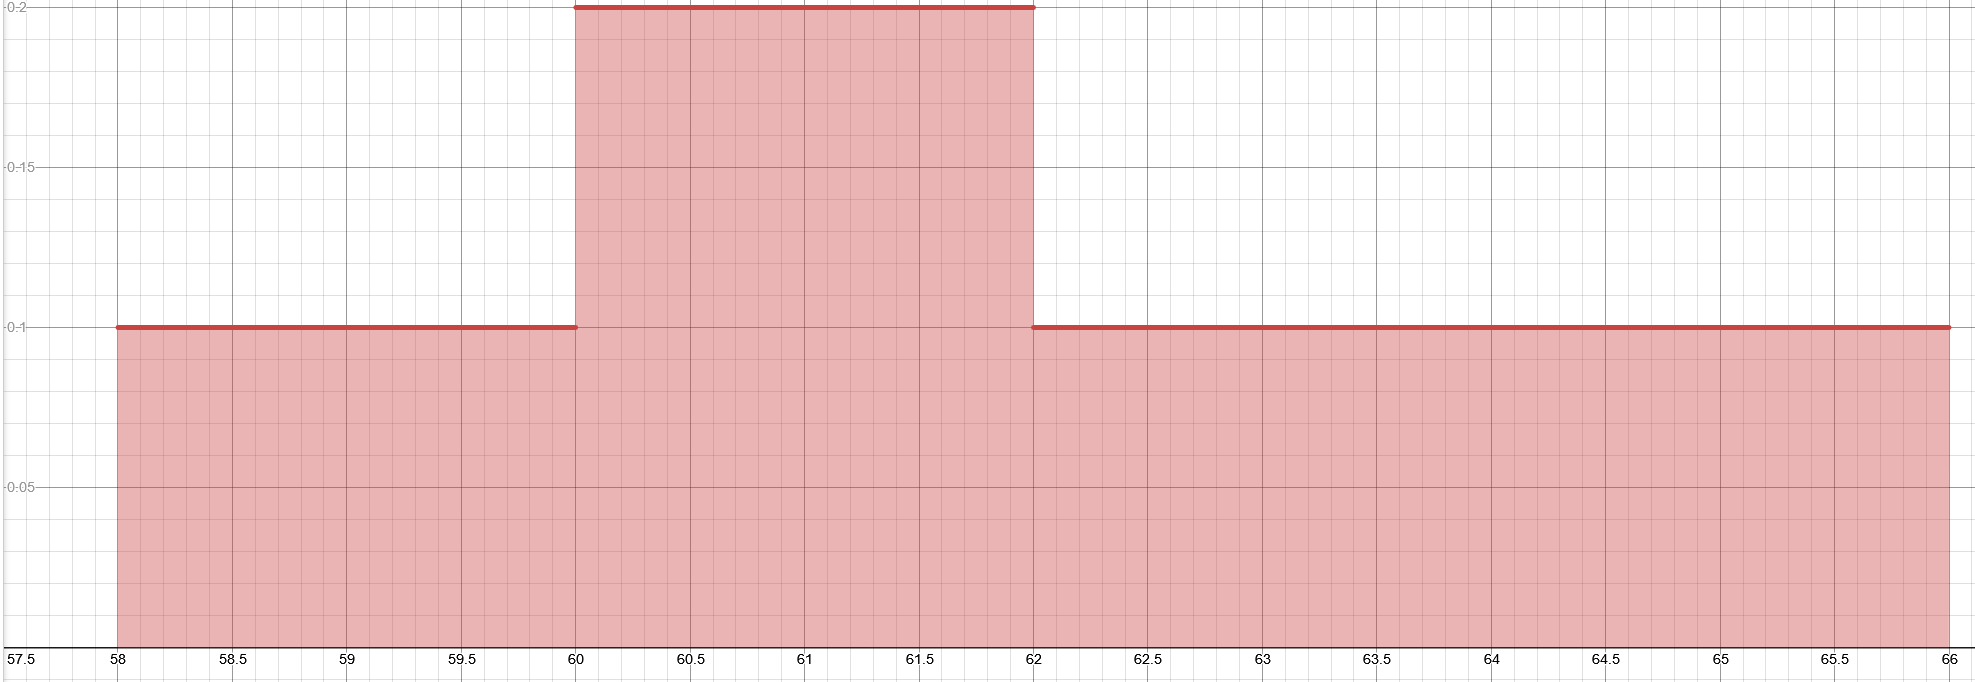
\includegraphics[scale=.35]{3a1.png}
    \caption{Distribution of Temperature Given Chad Being in the Office}
    \label{fig:my_label}
\end{figure}

\begin{figure}[h!]
    \centering
    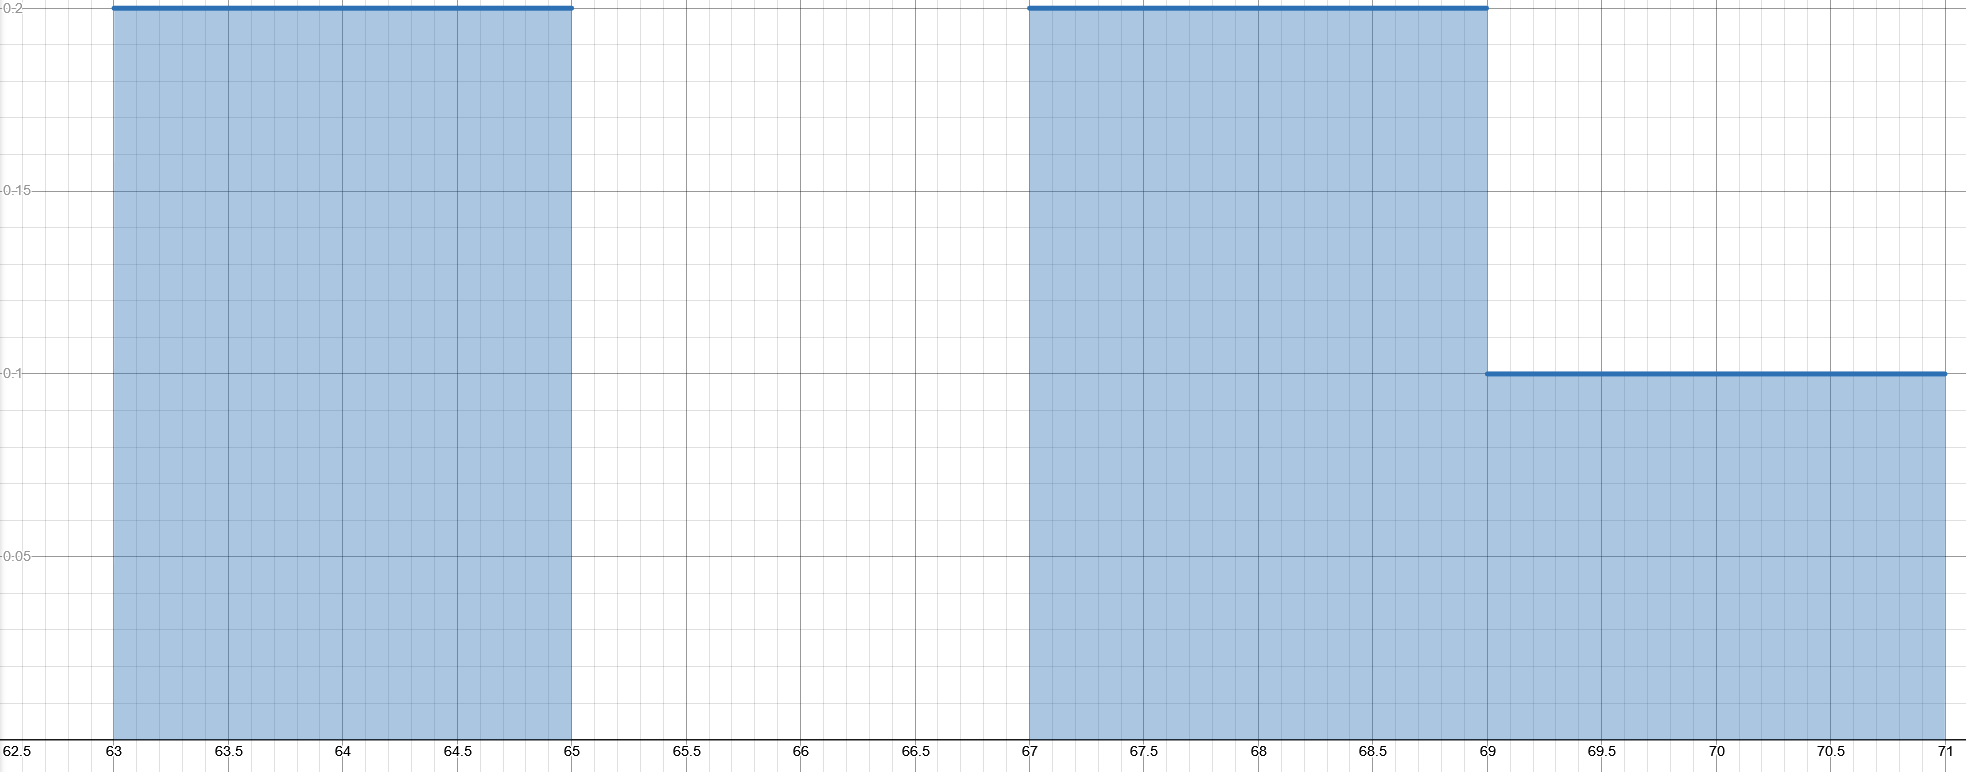
\includegraphics[scale=.35]{3a2.png}
    \caption{Distribution of Temperature Given No Chad the Office}
    \label{fig:my_label}
\end{figure}
\item We model the presence or not of Chad as a parameter $c$ ($c=1$ means he is present, $c=0$ that he is absent). If the temperature is 68$^{\circ}$, does a maximum-likelihood estimate of $c$ predict that Chad is in the office?
\subitem If the temperature is 68 degrees we conclude that he is not at the office. This is because we have no data points of chad being at the office when the temperature is 68 degrees, but we do have observed data of Chad being gone when temperature is 68 degrees. If we use the kernel density estimates we calculated, $P(68 \text{ degrees } | \text{ No Chad }) = .2$ and $P(68 \text{ degrees } | \text{ Chad })$ = 0. 
\item Now we take a Bayesian approach and model the presence or absence of Chad using a random variable $\rC$ which is equal to 1 if he is there and 0 if he is not. Estimate the pmf of $\rC$ from the data.
\subitem
If we take this approach we can estimate our parameters in the following way:
$$
    P(\text{Chad}) = \frac{\text{Observations of Chad}}
    {\text{Total Observations}}=\frac{10}{15} = \frac{2}{3}$$
    
    $$P(\text{No Chad}) =  \frac{\text{Observations of No Chad}}{\text{Total Observations}} = \frac{5}{15} = \frac{1}{3}
$$
\item If the temperature is 64$^{\circ}$, use the posterior distribution of $\rC$ to predict whether Chad is in the office
\subitem We can use Bayes rule to predict the to predict if chad is in the office given its 64$^{\circ}$.
\begin{equation}
    \begin{split}
        P(\text{Chad}|64^{\circ}) &= \frac{P(\text{Chad}) \times P(64^{\circ}|\text{Chad})}{P(64^{\circ})} \\
        P(\text{Chad}|64^{\circ})  &= \frac{P(\text{Chad}) \times P(64^{\circ}|\text{Chad})}{P(\text{Chad})P(64|\text{Chad}) + P(\text{No Chad})P(64|\text{No Chad})} \\
        P(\text{Chad}|64^{\circ})  &= \frac{\frac{2}{3}\times \frac{1}{10}}{(\frac{1}{3}\times \frac{2}{10}) + (\frac{2}{3}\times \frac{1}{10})} = \frac{1}{2} \\
        \text{And} & \\
        P(\text{No Chad}|64^{\circ}) &= 1 - P(\text{Chad}|64^{\circ}) = \frac{1}{2}
    \end{split}
\end{equation}
    

\item What problem do we run into if the temperature is 57$^{\circ}$? Explain how using parametric estimation may alleviate this problem.
\subitem The problem is if we have a temperature is 57$^{\circ}$ we have no observations or KDE density around that point, so we have no way of predicting whether or not Chad is in the office. Parametric models circumvent this, as they have a set distribution that real world data molds. If we used something like a Gaussian distribution, then there would be real, non negative, probability of Chad being in the office or not in the office at any given temperature. This is one way that parametric modeling can help model phenomena when you do not have much observational data.

\end{enumerate}

\item (Heart-disease detection)
A hospital is interested in developing a system for automatic heart-disease detection\footnote{A patient is deemed to suffer from heart disease if at least one of his or her major vessels is 50$\%$ narrower than it should be.}. Your task is to use the data in the \emph{heart\_disease\_data.npz}\footnote{The data in this problem, which was compiled from five hospitals in Hungary, Switzerland and the United States, is available at \url{http://archive.ics.uci.edu/ml/datasets/Heart+Disease}.  }  and complete the script\footnote{The script is avaiable at \url{https://github.com/cfgranda/prob_stats_for_data_science/blob/main/modeling_discrete_continous_data/heart_diseases_EXERCISE.ipynb} } to detect heart disease in patients. You model heart disease as a random variable $\rnd{h}$ that indicates whether the patient suffers from heart disease or not:
\begin{align*}
\rnd{h} = \begin{cases}
0 \quad \text{if patient does not suffer from heart disease},\\
1 \quad \text{if patient suffers from heart disease}.
\end{cases} 
\end{align*}
The available data contain the patient's sex, the type of chest pain experienced by the patient and the cholesterol of the patient. We model these quantities as the random variables $\rnd{s}$, $\rnd{c}$ and $\rnd{x}$ respectively, where
\begin{align*}
\rnd{s} & = \begin{cases}
0 \quad \text{if patient is female},\\
1 \quad \text{if patient is male},
\end{cases}\\
\rnd{c} &= \begin{cases}
0 \quad \text{if the pain is typical angina},\\
1 \quad \text{if the pain is atypical angina},\\
2 \quad \text{for other types of chest pain},\\
3 \quad \text{if there is no chest pain},
\end{cases}
\end{align*}
and $\rnd{x}$ is a continuous random variable.
\begin{enumerate}
\item Derive the MAP estimate of $\rnd{h}$ given $\rnd{s}$ and $\rnd{c}$ as a function of the pmf of $\rnd{h}$ ($ p_{\rnd{h}}$) and the conditional pmfs $p_{\rnd{s}|\rnd{h}}$ and $ p_{\rnd{c}|\rnd{h}}$. The MAP estimate is defined as the mode of the posterior distribution. Assume that if we know whether a patient is suffering from heart disease, the sex of the patient and the type of chest pain experienced by the patient are conditionally independent. 
%\emph{hw4q4.py}
\subitem
Since $\rnd{s}$ and $\rnd{c}$ are conditionally independent given $\rnd{h}$, we can express the probability of $\rnd{h}$ given $\rnd{c}, \rnd{s}$ as:
$$
    p(h|s,c) = \frac{P(h)P(s|h)P(c|h)}{P(s,c)}
$$
Now we can compute the MAP estimate of $h$ given $s,c$
$$
    MAP(h) = \begin{cases}
       0 & \ if \ P(1)P(s|1)P(c|1) < P(0)P(s|0)P(c|0) \\
       1 & \ Otherwise
    \end{cases}
$$
\item Complete the corresponding part of the script to estimate the necessary probability mass functions from the data. The training data consists of 218 patients and is provided in the arrays \emph{data["heart\_disease"]}, \emph{data["sex"]} and \emph{data["chest\_pain"]}. Apply the MAP decision rule you derived in part (a) to predict whether a group of 50 other patients, whose information is stored in the vectors \emph{data["sex\_test"]} and \emph{data["chest\_pain\_test"]}, suffer from heart disease. Calculate the error rate (i.e. the proportion of predictions that are incorrect) by comparing your results to \emph{data["heart\_disease\_test"]}, which indicates whether the patients suffer from heart disease or not.
\item Derive a MAP estimate of $\rnd{h}$ given $\rnd{s}$, $\rnd{c}$ and $\rnd{x}$ that only depends on the pmf of $\rnd{h}$ $ p_{\rnd{h}}$, the conditional pmfs $p_{\rnd{s}|\rnd{h}}(s|h)$ and $ p_{\rnd{c}|\rnd{h}}$ and the conditional pdf $f_{\rnd{x}|\rnd{h}}$, assuming that if we know whether a patient is suffering from heart disease,  the sex, type of chest pain and cholesterol level of the patient are all independent.
\subitem
Since $\rnd{s}$ and $\rnd{c}$ and \rnd{x} are conditionally independent given $\rnd{h}$, we can express the probability of $\rnd{h}$ given $\rnd{c}, \rnd{s}$ and \rnd{x} as:
$$
    p(h|s,c,x) = \frac{P(h)P(s|h)P(c|h)f(x|h)}{P(s,c)f(x|s,c)}
$$
Now we can compute the MAP estimate of $h$ given $s,c,x$
$$
    MAP(h) = \begin{cases}
       0 & \ if \ P(1)P(s|1)P(c|1)f(x|1) < P(0)P(s|0)P(c|0)f(x|0) \\
       1 & \ Otherwise
    \end{cases}
$$
\item You decide to model the cholesterol level of a patient conditioned on whether he or she suffers from heart disease as a Gaussian random variable. For both cases, complete the corresponding part of the script to obtain the ML estimates of the conditional distributions from the data in \emph{cholesterol} and compare the estimated pdf to the histogram of the data. 
\item Complete the corresponding part of the script to apply your MAP decision rule incorporating the cholesterol data and compute the new error rate (using the cholesterol rates of the 50 new patients, stored in \emph{data["cholesterol\_test}"]. %Do you trust this result?
\item We have made some conditional independence assumptions that do not necessarily hold. Another option would have been to estimate the joint distribution of all the random variables from the data. Is this a good idea? % Why? (Hint: The answer is not necessarily yes or no. Reason about what happens if we have a lot of data available or not.)
\subitem
We honestly don't have much data, with only 218 observations estimating a joint distribution for all possible combinations of features would be intractable. I personally don't think that it would be advisable to estimate all of the joint distributions. When it comes to real world modelling, we must introduce some assumptions to fight off the curse of dimentionality. Otherwise, we would never be able to model anything. It's better to have models that are wrong, but useful, rather than no models at all. 
\end{enumerate}
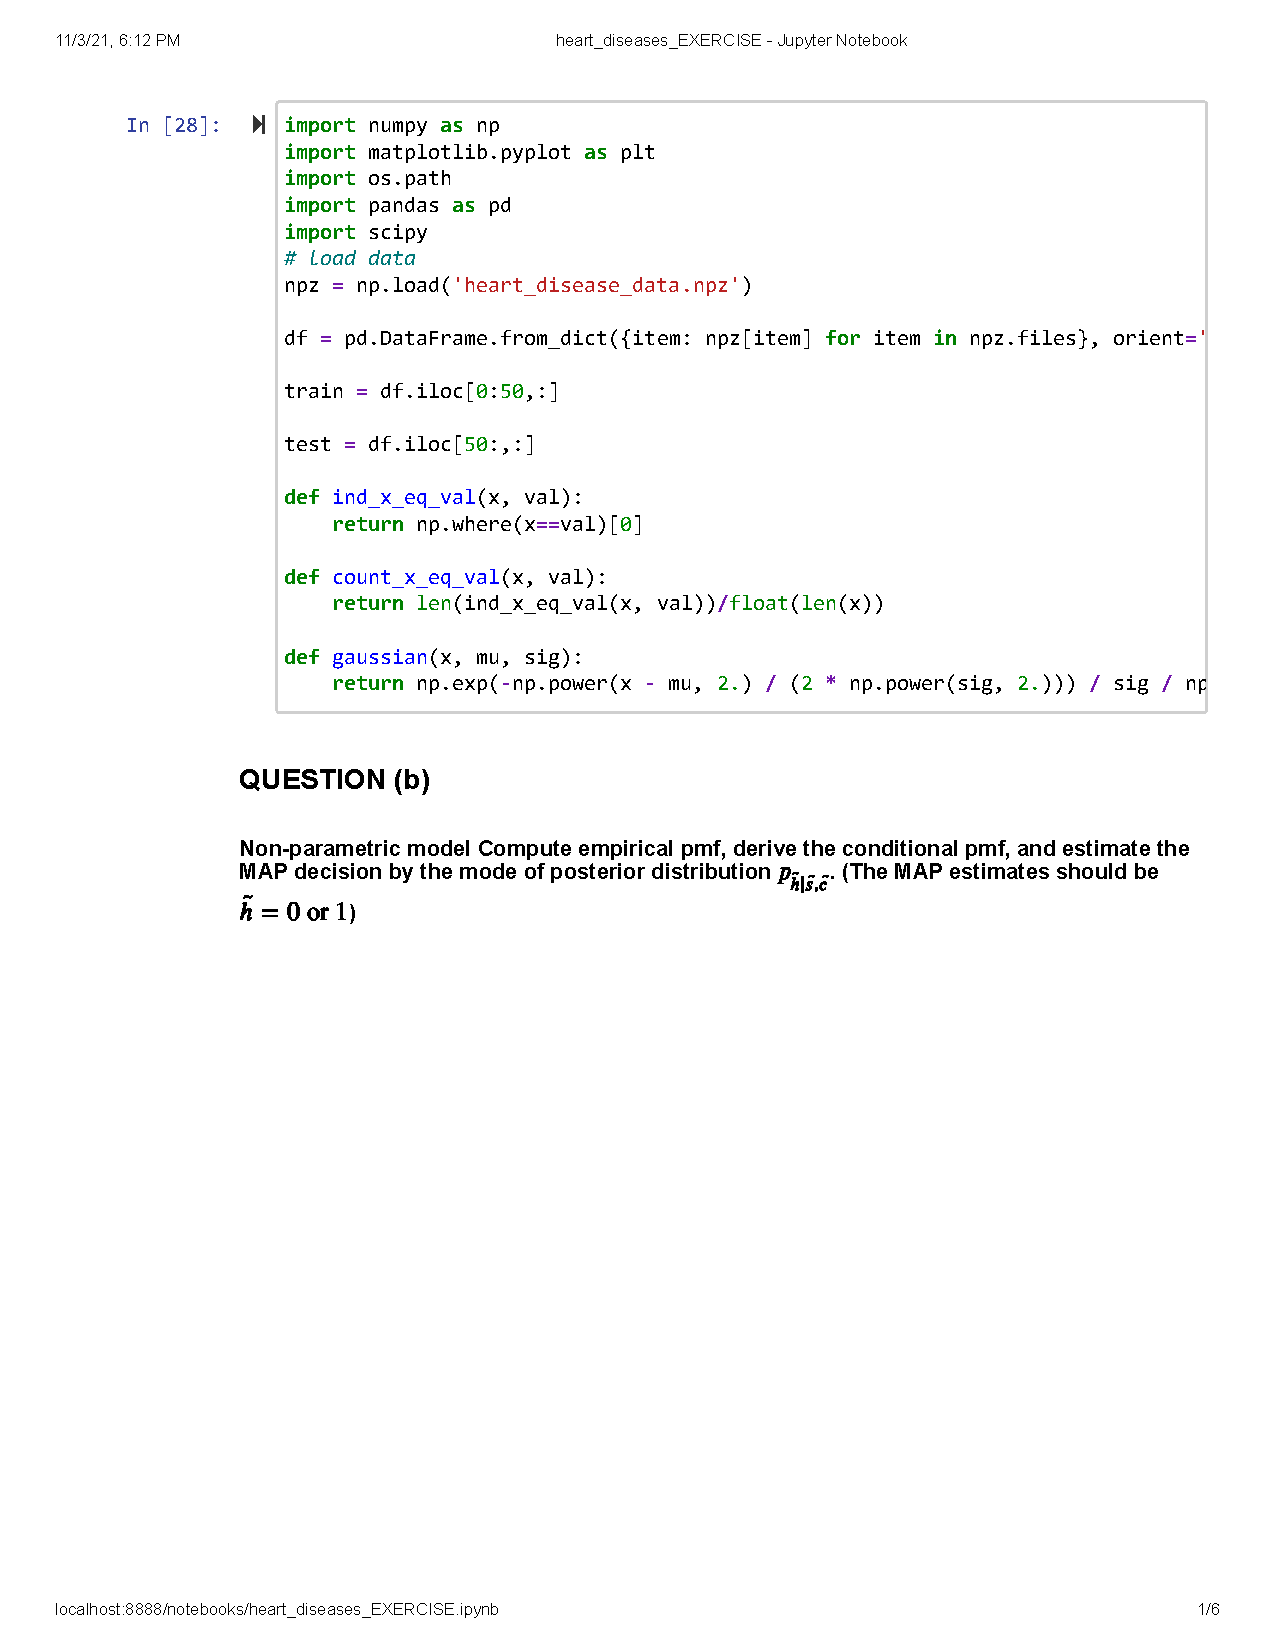
\includepdf[pages=-]{hw6 python.pdf}
\end{enumerate}
\end{document}
